\item In the arrangement shown in Fig. 1.16 the bodies have masses \( m_0, m_1, m_2 \), the friction is absent, the masses of the pulleys and the threads are negligible. Find the acceleration of the body \( m_1 \). Look into possible cases.
    \begin{center}
        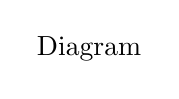
\begin{tikzpicture}
            \node at (0, 0) {Diagram};
        \end{tikzpicture}
    \end{center}

\begin{solution}
    \begin{center}
        \begin{tikzpicture}
            \pic at (0, 0) {frame=3cm};
        \end{tikzpicture}
    \end{center}
    
    \begin{align*}
        \intertext{Let us write Newton’s second law for masses \(m_1\) and \(m_2\) and moving pulley in vertical direction along positive \(x\)-axis (see figure):}
        m_1g - T &= m_1w_{1x} \\
        m_2g - T &= m_2w_{2x} \\
        T_1 - 2T &= 0 \quad (\text{as } m = 0)\\
        \intertext{or}
        T_1 &= 2T \\
        \intertext{Again using Newton’s second law in projection form for mass \(m_0\) along positive \(x_1\) direction (see figure), we get}
        T_1 &= m_0w_0 \\
        \intertext{The kinematic relationship between the accelerations of masses given in terms of projection on the \(x\)-axis}
        w_{1x} + w_{2x} &= 2w_0 \\
        \intertext{Simultaneous solution of the obtained five equations yields, in vector form}
        \vec{w}_1 &= \dfrac{[4m_1m_2 + m_0 \left(m_1 - m_2\right)]g}{4m_1m_2 + m_0\left(m_1 + m_2\right)}
    \end{align*}
\end{solution}
